\documentclass[12pt,a4paper]{report}
\usepackage[utf8]{inputenc} % un package
\usepackage[T1]{fontenc} % un second package
\usepackage[francais]{babel} % un troisième package
\usepackage{color} % Package de la couleur
\usepackage{verbatim}
\usepackage{moreverb}
\usepackage{amsmath}
\usepackage{amsfonts}
\usepackage{amssymb}
\usepackage{graphicx}
\usepackage[top=2cm, bottom=2cm, left=2cm, right=2cm]{geometry}
\author{IMA World Health Web Developer Team}
\title{
\includegraphics[width=12cm]{ima.png} \\Hospital Management System\\ (HMS) \\ Manuel d'utilisation}

\begin{document}
%Page de garde
\maketitle 
\chapter{Présentation}
\section{Accès au système}
\large{Pour accéder au système, la première de chose à faire est de lancer un navigateur web, en suite saisir l'adresse web de l'application dans la barre d'adresse du navigateur.}

La première interface de l'application est un formulaire qui demande à chaque utilisateur de pouvoir fournir le login, le mot de passe mais  aussi le projet dont il sont assigné, comme le montre le formulaire ci-dessous.
\begin{figure}[h]
\begin{center}
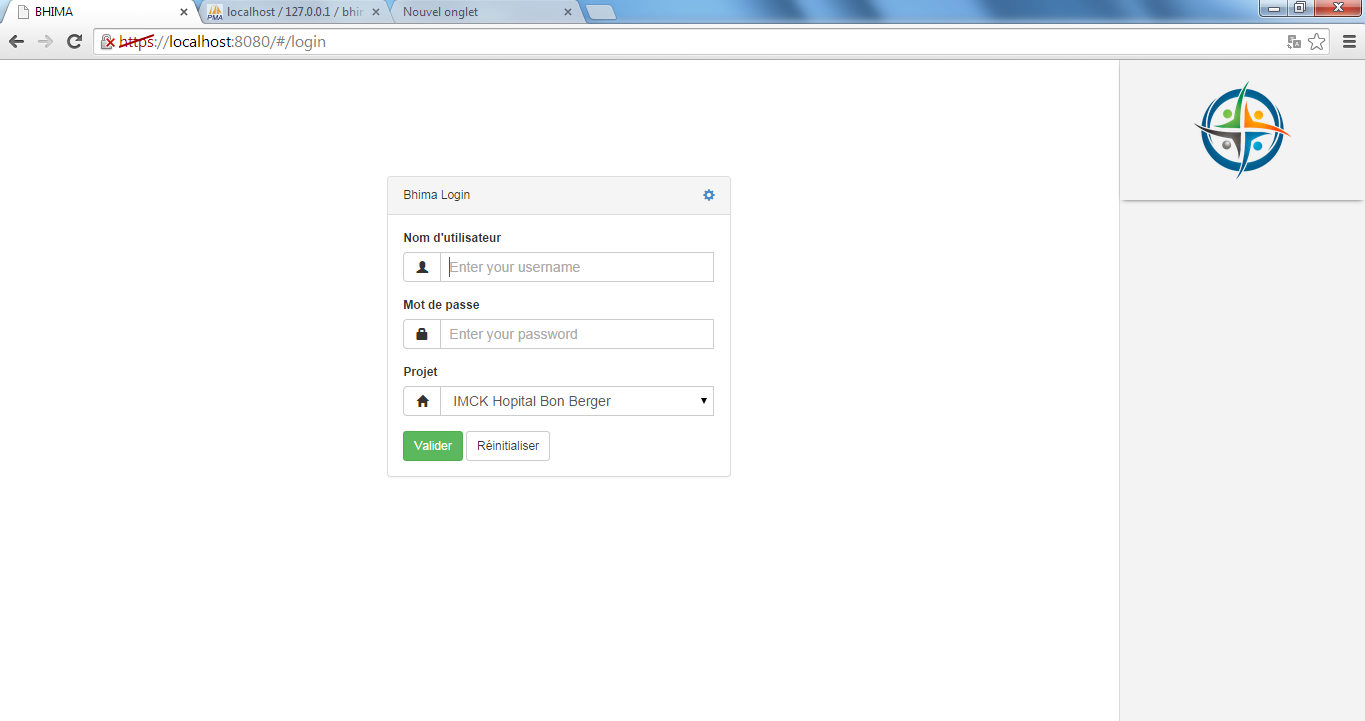
\includegraphics[width=12cm]{pic/login.png}
\end{center}
\caption{Page d'identification et authentification des utilisateurs}
\label{Page d'identification et authentification des utilisateurs}
\end{figure}
\\ L'accès au système n'est garanti que pour ceux qui possèdent un compte utilisateur, si l'utilisateur est authentifié alors il sera dirigé vers l'interface principale de l'application qui se présente de la manière suivante.
\newpage
\begin{figure}[h]
\begin{center}
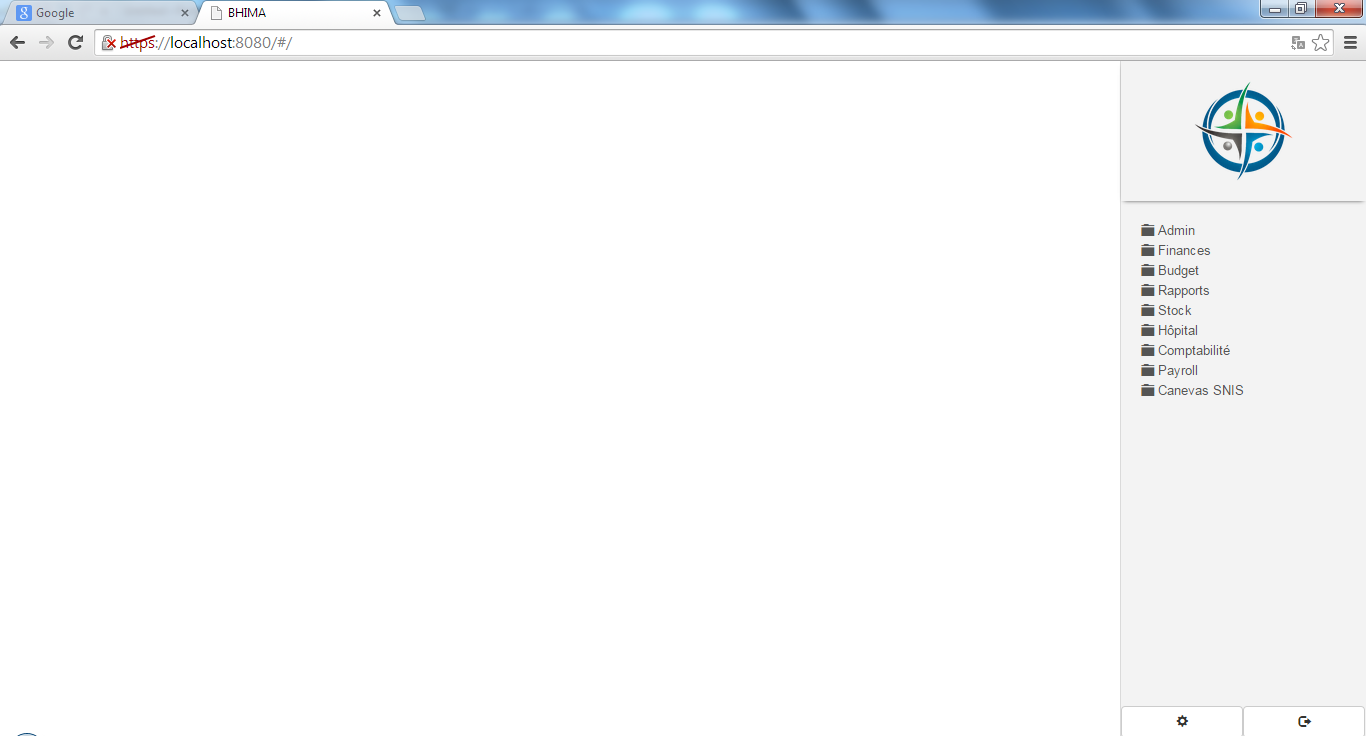
\includegraphics[width=10cm]{pic/mainInterface.png}
\end{center}
\caption{Interface principale de l'application}
\label{Interface principale de l'application}
\end{figure} 
Dans sa partie gauche de la figure ci-dessous on retrouve le logo IMA World Heath Ainsi que l'arborescence qui représente le niveau d'accès de l'utilisateur. En dessous de l'arborescence figure deux boutons, le premier 
\includegraphics[scale=0.5]{pic/lang.png} permet de changer de langue et le second 
\includegraphics[scale=0.5]{pic/logout.png} permet de ce déconnecté du système.

\begin{figure}[h]
\begin{center}
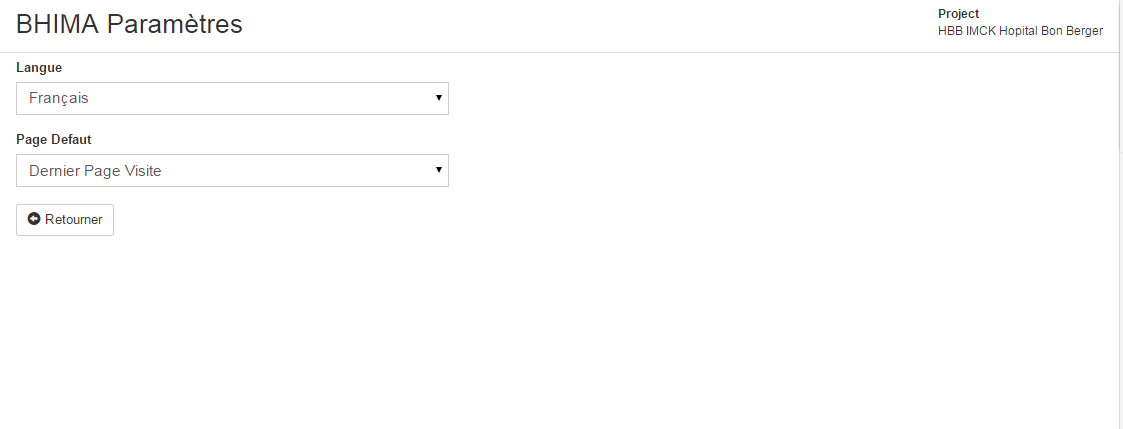
\includegraphics[width=10cm]{pic/changeLang.png}
\end{center}
\caption{Interface principale pour le changement de langue}
\label{Interface principale pour le changement de langue}
\end{figure} 
\newpage
\section{Les modules du système HMS}
Le système d'information HMS possède plusieurs modules qui sont représenté par l'arborescence ci-dessous.
\begin{figure}[h]
\begin{center}
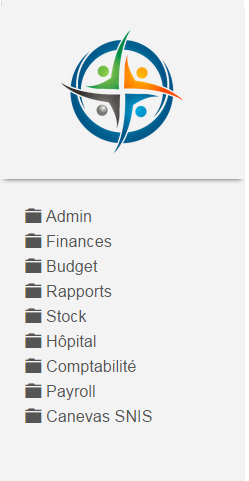
\includegraphics[width=4.5cm]{pic/arbo.png}
\end{center}
\caption{Arborescence du système}
\label{Arborescence du système}
Voici les différentes rubriques qui existent dans le système:
\end{figure} 
% Liste des modules
\begin{itemize}
\item Admin. %•
\item Finance
\item Budget
\item Rapports
\item Stock
\item Hôpital
\item Payroll
\item Comptabilité
\item Canevas SNIS
\end{itemize}
Nous allons à présent détailler chacun d'entre eux.
\newpage
%%%%%%%%%%%%%%%%%%%%%%%%%%%%%%%%%%%%%%%%%%%%%
%   MODULES DU SYSTEMES                     %
%%%%%%%%%%%%%%%%%%%%%%%%%%%%%%%%%%%%%%%%%%%%%
    
\chapter{Le module Admin}        
%////////////////////////////////////////////////%
% MODULE ADMIN
Le module admin est compose des sous modules qui permettent d'administrer le système. La figure ci-dessous représente avec exactitude ce module avec les différents sous éléments.
\begin{figure}[h]
\begin{center}
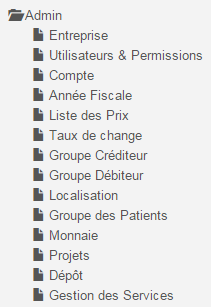
\includegraphics[width=4cm]{pic/s_admin.png}
\end{center}
\caption{Le module Admin et ses sous modules}
\label{Le module Admin et ses sous menus}
\end{figure} 

\section{Taux d'échange}
Le module de taux de change, donne la possibilité de définir le taux d'échange du jour. Par souci d'intégrité des données, Le taux d'échange doit être défini chaque jour.


\begin{figure}[h]
\begin{center}
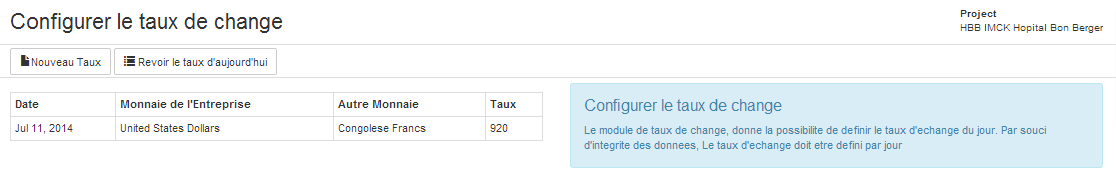
\includegraphics[width=16cm]{pic/FormulaireConfigRate.png}
\end{center}
\caption{Formulaire permettant de configurer le taux de change}
\label{Formulaire permettant de configurer le taux de change}
\end{figure}

\subsection{Nouveau Taux}
Lorsque l'utilisateur click sur le bouton 
\includegraphics[scale=0.7]{pic/NouveauTaux.png}
 Le formulaire ci-après apparait.

\begin{figure}[h]
\begin{center}
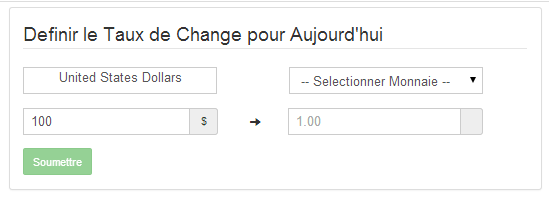
\includegraphics[width=12cm]{pic/DefinirTaux.png}
\end{center}
\caption{Formulaire permettant de definir le taux}
\label{Formulaire permettant de definir le taux}
\end{figure}
\begin{itemize}
\item \textbf{United States Dollars}: est la monnaie principale de l'application, l'équivalence avec les autres monnaie ne doit se faire qu'avec la somme de 100 Dollars,
\item \textbf{Sélectionner Monnaie}: Affiche la liste des monnaies qui existe dans le système et la zone de saisie qui se retrouve en bas permet de préciser l'équivalence avec la monnaie principale.
\end{itemize}
Après avoir renseigné ce deux champs, un clique sur le bouton \textbf{Soumettre} permet de définir les taux du jour.

\subsection{Revoir le taux d'aujourd'hui}
Un clic sur le bouton 
\includegraphics[scale=0.7]{pic/RevoirTaux.png} permet d'afficher toutes les informations sur le taux du jour, comme la montre la figure ci-dessous.
\begin{figure}[h]
\begin{center}
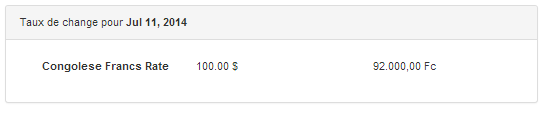
\includegraphics[width=12cm]{pic/ShowRate.png}
\end{center}
\caption{Aperçue du taux du jour}
\label{Aperçue du taux du jour}
\end{figure}

\newpage
\chapter{Le module finance}        
%////////////////////////////////////////////////%
Le module finance est composé des sous modules qui permettent d'administrer le finance. La figure ci-dessous représente avec exactitude ce module avec ses différents sous éléments.

\begin{figure}[h]
\begin{center}
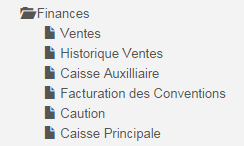
\includegraphics[width=6cm]{pic/FinanceArbo.png}
\end{center}
\caption{Arborescence du module Finance}
\label{Arborescence du module Finance}
\end{figure}

\section{Caisse Principale}
Le module caisse principale, est l'un des principaux modules de cette application, ce module permet d'administrer les recettes ainsi que les dépenses qui s'oppere au sein de l'organisation.

Son interface principale se présente de la manière que voici.

\begin{figure}[h]
\begin{center}
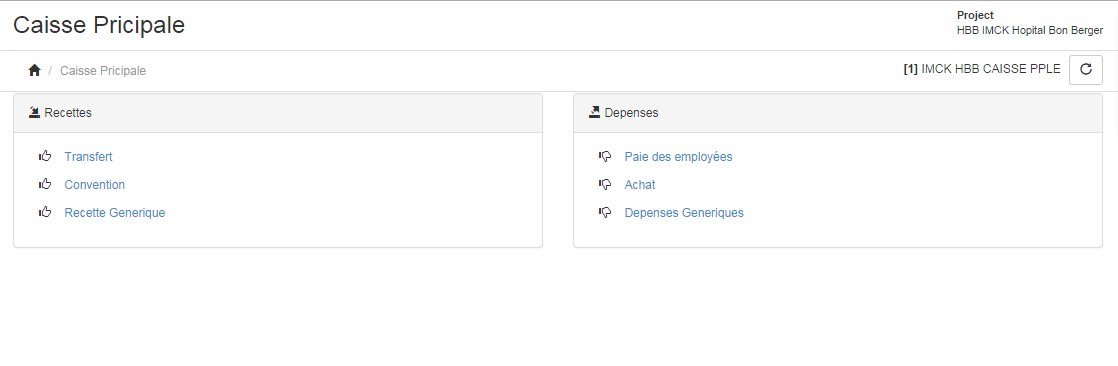
\includegraphics[width=14cm]{pic/caissePrincipale.png}
\end{center}
\caption{Interface principale de la caisse principale}
\label{Interface principale de la caisse principale}
\end{figure}

Cette interface possède deux menus, le premier \textbf{Recettes} et le second \textbf{Dépenses}

\subsection{Recettes : Transfert}
Ce module permet de faire le transfert de fond d'une caisse à une autre, son interface d'utilisation est simple et se présente de la manière suivante.

\begin{figure}[h]
\begin{center}
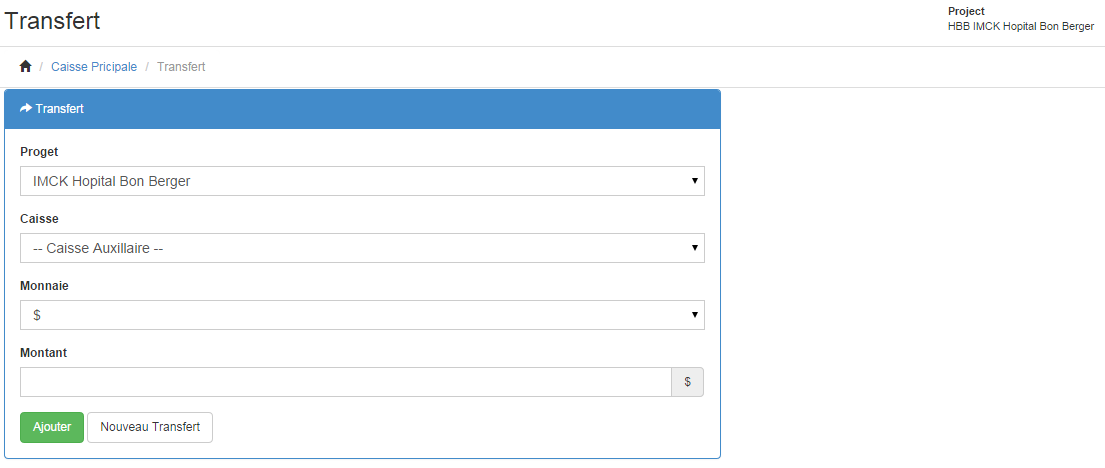
\includegraphics[width=14cm]{pic/Transfert.png}
\end{center}
\caption{Interface principale du module transfert}
\label{Interface principale du module transfert}
\end{figure}

Voici les différents éléments qui composent cet interface.

\begin{itemize}
\item \textbf{Projet}: permet de préciser dans quelle projet s'effectue cet opération. \\
\item \textbf{Caisse}: permet de préciser dans quelle caisse est allouée le fond .\\
\item \textbf{Monnaie}:Pour la monnaie utiliser pour la transaction \\
\item \textbf{Montant}: Pour le motant du transfert\\
\end{itemize}
Après avoir renseigner les différents éléments de ce formulaire, il suffit de cliquer sur le bouton \textbf{Ajouter} pour réaliser le transfert de fond, et pour toute opération de transfert le système générera un reçu.

\newpage
\subsection{Recettes : Convention}
Ce modules permet à des entreprises conventionnées de pouvoir payer les factures de leurs agents ou bien des personnes aux quelles ils prennent en charge, son interface principale se présente de la sorte.

\begin{figure}[h]
\begin{center}
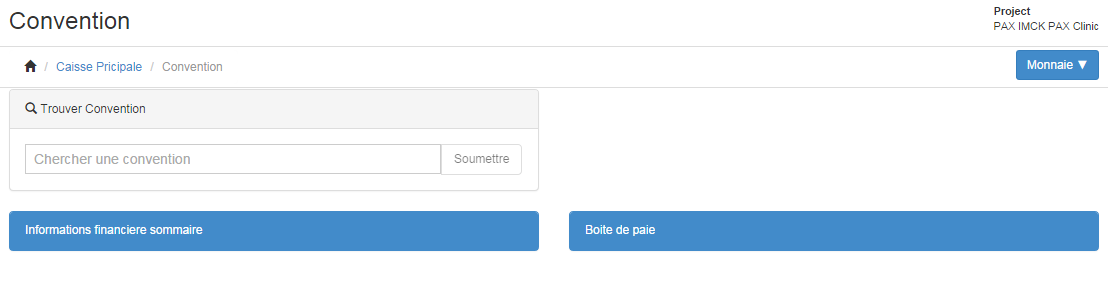
\includegraphics[width=14cm]{pic/conventionMenu.png}
\end{center}
\caption{Interface principale du module Convention}
\label{Interface principale du module Convention}
\end{figure}

Dans le coin superieur gauche il y'a un bouton qui permet de préciser la monnaie qui sera utilisée lors de l'opération du paiement.

En suite il y'a une zone de recherche qui permet de rechercher la convention qui procéder aux paiements, une fois qu'on a retrouver la dite convention, il suffit de cliquer sur le bouton soumettre pour que s'affiche la situation des tous les patients appartenant à la convention ou bien au groupe débiteur choisi, comme le montre la figure ci-après.


\begin{figure}[h]
\begin{center}
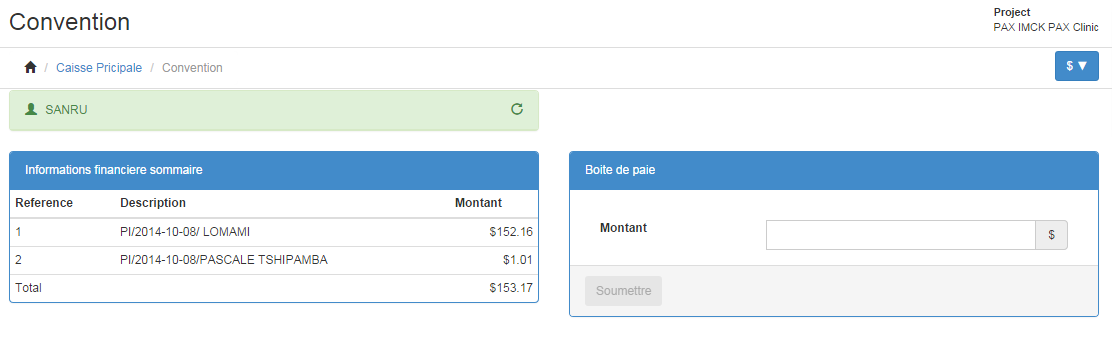
\includegraphics[width=14cm]{pic/conventionMenu2.png}
\end{center}
\caption{Illustration d'un cas de paiement pour un groupe débiteur dont seulement deux patients ont été facturé}
\label{Illustration d'un cas de paiement pour un groupe débiteur dont seulement deux patients ont été facturé}
\end{figure}
 
Dans cette interface nous avons un tableau à gauche qui renseigne sur les informations financières sommaire et en bas du tableau, la totalité de ce que doit le groupe débiteur à l'hôpitale, la zone boite de paiement permet de préciser le montant à payer.

une fois que cette opération est effectué un spéciment de reçu pour les conventions sera généré automatiquement par le système.


\newpage
\subsection{Recettes : Recette Générique}
Les modules recette générique est un module qui a été ajouter au système enfin de pour traquer toutes les recettes générées par l'organisation en dehors des activités liées à l'hôpital, pour l'enregistrement de ce genre des recettes, il faudrait prémierement choisir le compte qui sera utiliser pour l'enregistrement des recettes.

l'interface principale de ce module se présente comme ceci.

\begin{figure}[h]
\begin{center}
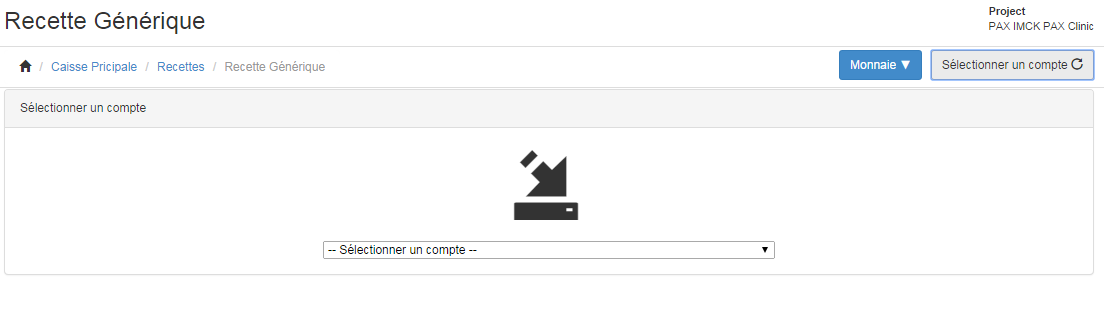
\includegraphics[width=14cm]{pic/recetteGen.png}
\end{center}
\caption{Interface principale permettant de sélectionner un compte}
\label{Interface principale permettant de sélectionner un compte}
\end{figure}

Sur cette interface on aussi un bouton qui permet de préciser la monnaie, et si un compte est déjà choisi par défaut on a la possibilité de la modifier grace au bouton \textbf{Sélectionner un compte}

Après avoir choisi un compte, un deuxième interface apparait, cet interface possède un formulaire qui permet de renseigner les différentes information liée à l'activitité qui a généré une recette telle que la date de la réalisation de la recette, le label ou bien la désignation de la recette, le montant de la recette, il existe aussi un champ \textbf{Référence document ID} qui permet d'attribuer un identifiant unique à l'opération d'enregistrement des recettes.

\begin{figure}[h]
\begin{center}
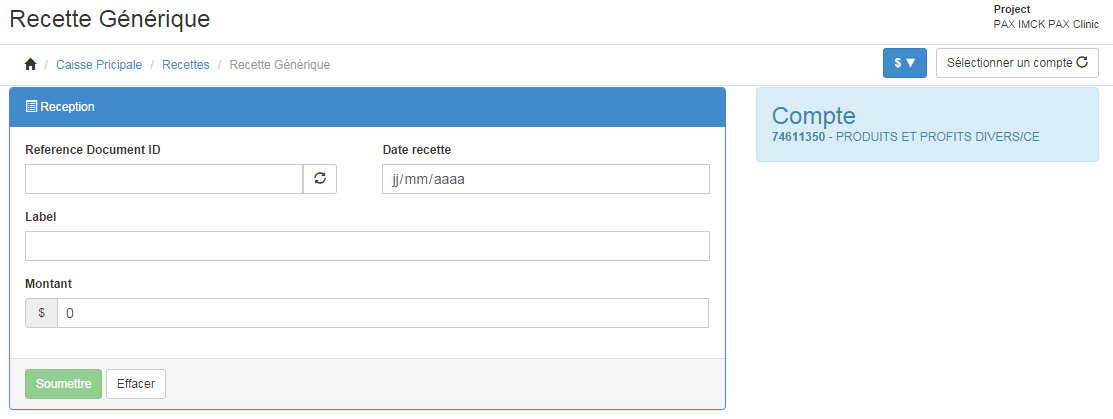
\includegraphics[width=14cm]{pic/recetteGen2.png}
\end{center}
\caption{Interface principale permettant d'enregistrer une recette générique}
\label{Interface principale permettant d'enregistrer une recette générique}
\end{figure}

Dans la zone qui retrouve à droite renseigne sur le compte qui est utilé pour l'opération. Il suffit de cliquer sur le bouton soumettre pour confirmer l'enregistrement d'une recette générique.

\subsection{Dépenses : Paie des employés}
Le module paie des employées permet permet de déterminer les différentes éléments qui seront pris en charge lors du processus de paiement des employés, ce modules est composé d'autre modules qui sont Payroll Multiple, Paiement Taxes et Paiement taxes entreprise. Son interface principale se présente de cette façon.


\begin{figure}[h]
\begin{center}
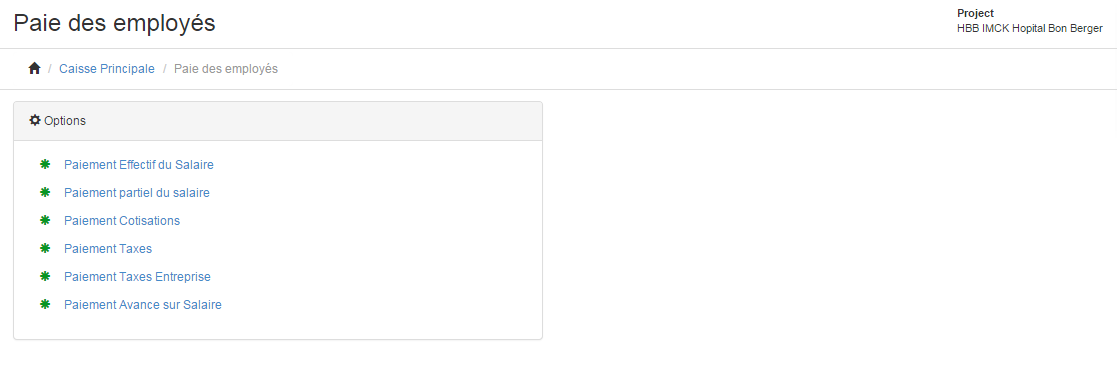
\includegraphics[width=14cm]{pic/paieEmp.png}
\end{center}
\caption{Interface principale du module paie des employés}
\label{Interface principale du module paie des employés}
\end{figure}


\subsection{Dépenses : Paie des employés : Paiement Taxes}
Le module paiement des taxes n'est utilisable que si il existe une période de paiment pour laquelle ce module n'est pas encore utilisé. ce module dispose ainsi d'une interface principale possédant une liste de choix.

\begin{figure}[h]
\begin{center}
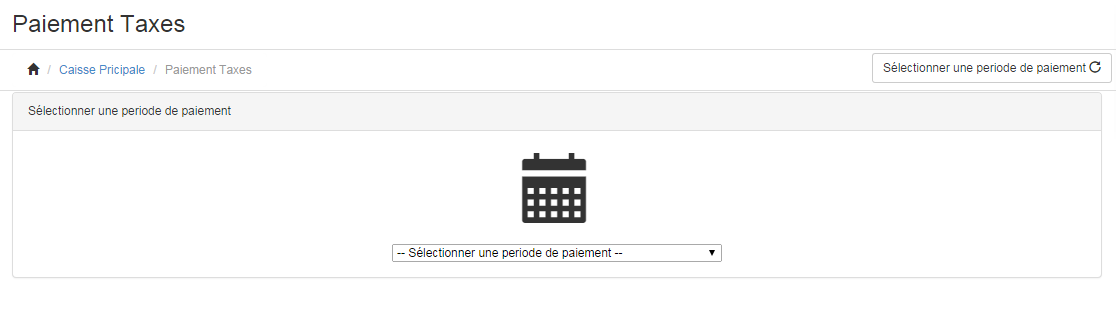
\includegraphics[width=14cm]{pic/PaieTaxes.png}
\end{center}
\caption{Interface principale permettant sélectionner une période de paiement}
\label{Interface principale permettant sélectionner une période de paiement}
\end{figure}

Une fois qu'une période de paiement est choisi, l'utilisateur est alors dirigé vers une interface principale du paiement de taxes. Cette interface se présente de la manière suivante.

\begin{figure}[h]
\begin{center}
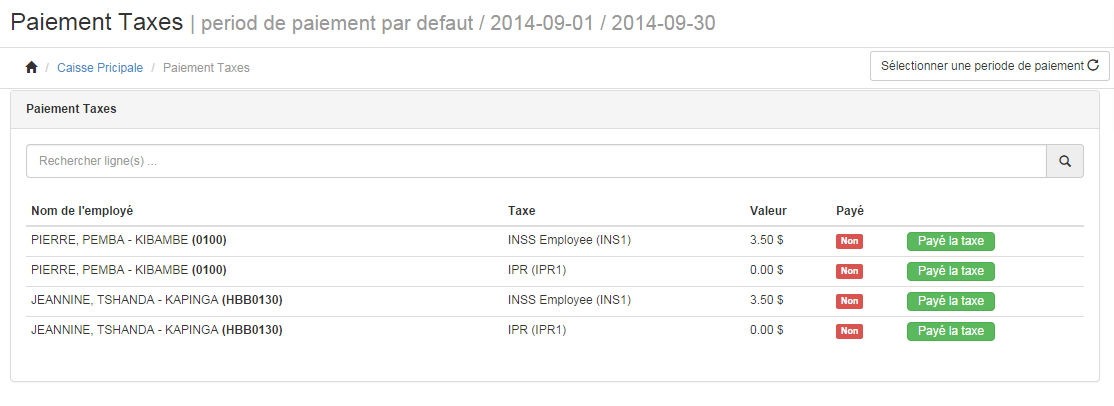
\includegraphics[width=14cm]{pic/PaieTaxes2.png}
\end{center}
\caption{Interface principale permettant de confirmer le paiement}
\label{Interface principale permettant de confirmer le paiement}
\end{figure}


Voici les différents éléments de l'interface. Un bouton sélectionner une période de paiement qui permet de revenir vers l'interface permettant de choisir une période de paiement, une barre de recherche permettant de filtrer les différents éléments composant le tableau des employés ainsi que des différentes taxes.

Le tableau est divisé en colonne, il existe le nom des employés, les types de taxes, la valeur, le status du paiement qui par défaut est 
\includegraphics[scale=0.7]{pic/NonTaxes.png} si la taxe n'est pas encore payée et 
\includegraphics[scale=0.7]{pic/OuiTaxes.png} si elle est payée. pour confirmer le paiement d'une taxe, il faudrait cliquer sur le bouton 
\includegraphics[scale=0.7]{pic/PayeTaxe.png}
\newpage
\subsection{Dépenses : Paie des employés : Paiement Taxes Entreprise}
Le module paiement des taxes Entreprise est similaire à celui permettant le paiement de taxes,  ce module n'est utilisable que si il existe une période de paiement pour laquelle ce module n'est pas encore utilisé. ce module dispose ainsi d'une interface principale possédant une liste de choix.

\begin{figure}[h]
\begin{center}
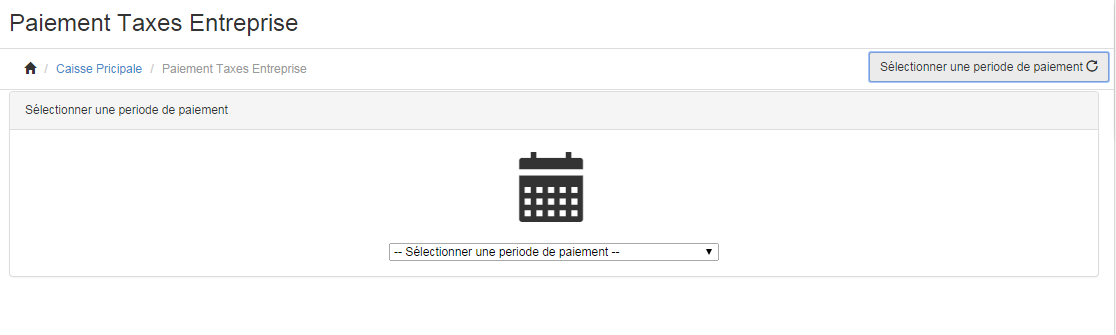
\includegraphics[width=14cm]{pic/PaieTaxesEntre.png}
\end{center}
\caption{Interface principale permettant sélectionner une période de paiement}
\label{Interface principale permettant sélectionner une période de paiement}
\end{figure}

Une fois qu'une période de paiement est choisi, l'utilisateur est alors dirigé vers une interface principale du paiement de taxes de l'entreprise. Cette interface se présente de la manière suivante.

\begin{figure}[h]
\begin{center}
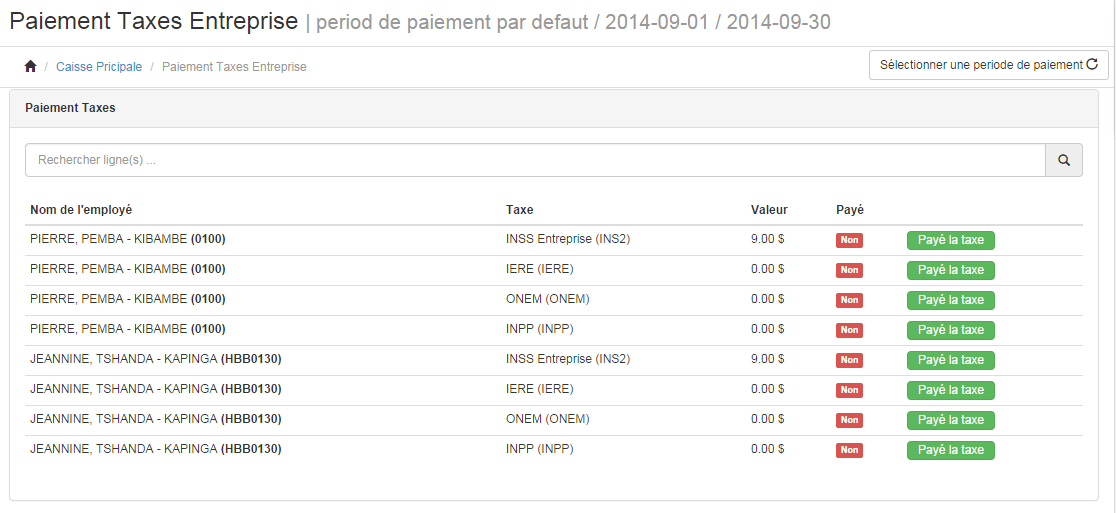
\includegraphics[width=14cm]{pic/PaieTaxesEntre2.png}
\end{center}
\caption{Interface principale permettant de confirmer le paiement}
\label{Interface principale permettant de confirmer le paiement}
\end{figure}


Voici les différents éléments de l'interface. Un bouton sélectionner une période de paiement qui permet de revenir vers l'interface permettant de choisir une période de paiement, une barre de recherche permettant de filtrer les différents éléments composant le tableau des employés ainsi que des différentes taxes.

Le tableau est divisé en colonne, il existe le nom des employés, les types de taxes, la valeur, le status du paiement qui par défaut est 
\includegraphics[scale=0.7]{pic/NonTaxes.png} si la taxe n'est pas encore payée et 
\includegraphics[scale=0.7]{pic/OuiTaxes.png} si elle est payée. pour confirmer le paiement d'une taxe, il faudrait cliquer sur le bouton 
\includegraphics[scale=0.7]{pic/PayeTaxe.png}

\subsection{Dépenses : Achat}
Ce module permet de faire sortir l'argent dans la caisse principale lors qu'un ordre d'achat a été établi, voici un apperçu de l'interface du modules Achat.

\begin{figure}[h]
\begin{center}
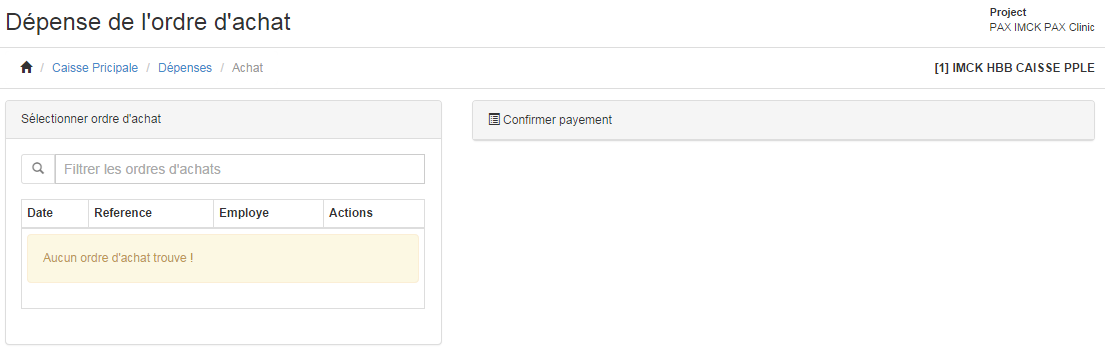
\includegraphics[width=14cm]{pic/Achat.png}
\end{center}
\caption{Interface principale du module Achat}
\label{Interface principale du module Achat}
\end{figure}

Dans l'interface qui est illustrée, aucun ordre d'achat n'est encore éffectué, mais au cas où il existe des ordres d'achat l'interface se présente de la manière suivante.

\begin{figure}[h]
\begin{center}
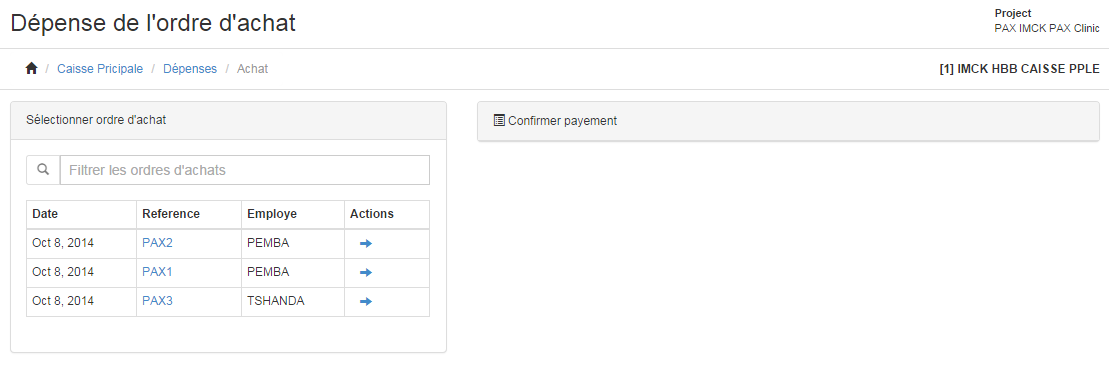
\includegraphics[width=14cm]{pic/Achat2.png}
\end{center}
\caption{Module Achat, avec des ordres d'achat}
\label{Module Achat, avec des ordres d'achat}
\end{figure}

On peut remarquer un tableau des différents ordres d'achat qui ne sont pas encore payer, ainsi qu'une permettant de filtrer les ordres d'achat. 

\newpage
Pour que la caisse puisse payer un ordre d'achat il faudrait cliquer sur le bouton 
\includegraphics[scale=0.7]{pic/SelectedPOrder.png} d'un ordre d'achat, cet action activera la zone permettant de commencer le processus de paiement, dans cette nouvelle interface on retrouvera les informations rélatives à l'ordre d'achat, un bouton permettant de confirmer le payement de l'ordre d'achat ainsi que celui permettant d'annuler un ordre d'achat.

\begin{figure}[h]
\begin{center}
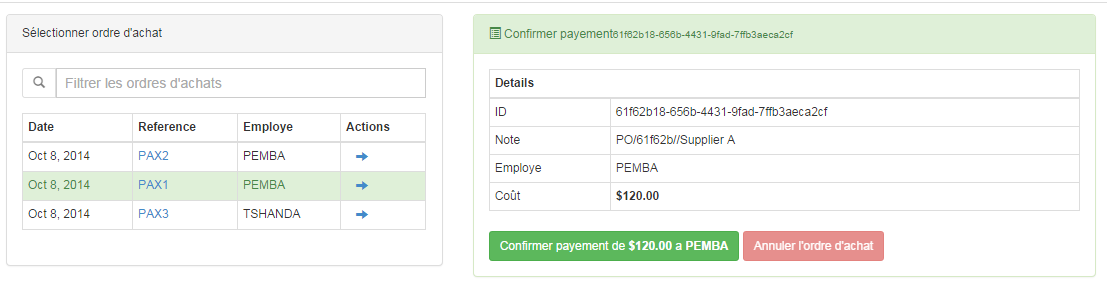
\includegraphics[width=14cm]{pic/ConfOrdreAchat.png}
\end{center}
\caption{Illustration de l'interface de confirmation de l'ordre d'achat}
\label{Illustration de l'interface de confirmation de l'ordre d'achat}
\end{figure}

Pour chaque ordre d'achat une preuve de paiement est directement produite par le système.

\begin{figure}[h]
\begin{center}
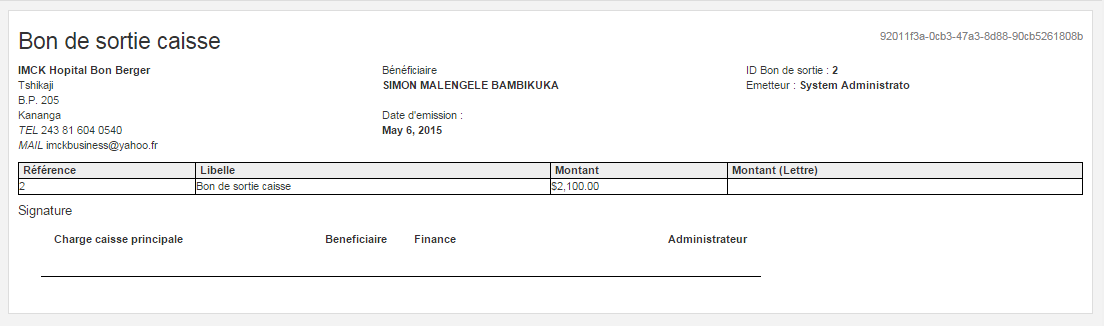
\includegraphics[width=14cm]{pic/PreuvePaiement.png}
\end{center}
\caption{Apperçue d'un ordre de paiement}
\label{Apperçue d'un ordre de paiement}
\end{figure}

\subsection{Dépenses : Dépenses Génériques}
Les modules dépenses génériques permet de tracquer tous les cas des dépenses de fonds au niveau de la caisse principale. l'interface principale de ce module est constituée d'une liste de choix qui permet de préciser le compte concerné par la dépence.
Voici l'illustration de cet interface.

\begin{figure}[h]
\begin{center}
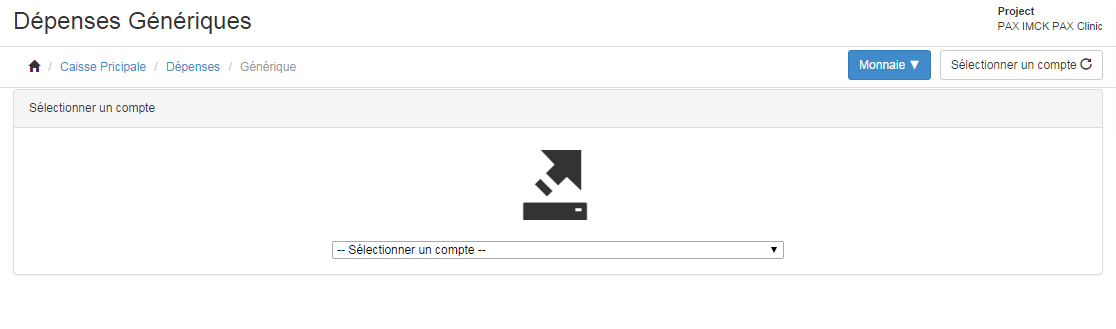
\includegraphics[width=14cm]{pic/DepenseGen.png}
\end{center}
\caption{Apperçue de l'interface principale du module Dépenses Génériques}
\label{Apperçue de l'interface principale du module Dépenses Génériques}
\end{figure}

Sur cette interface on aussi un bouton qui permet de préciser la monnaie, et si un compte est déjà choisi par défaut on a la possibilité de la modifier grace au bouton \textbf{Sélectionner un compte}

Après avoir choisi un compte, un deuxième interface apparait, cet interface possède un formulaire qui permet de renseigner les différentes information liée à l'activitité qui a nécéssitée une dépensetelle que la date, le label ou bien la désignation de la dépense, le montant de la dépense, il existe aussi un champ \textbf{Référence document ID} qui permet d'attribuer un identifiant unique à l'opération d'enregistrement des dépenses.

\begin{figure}[h]
\begin{center}
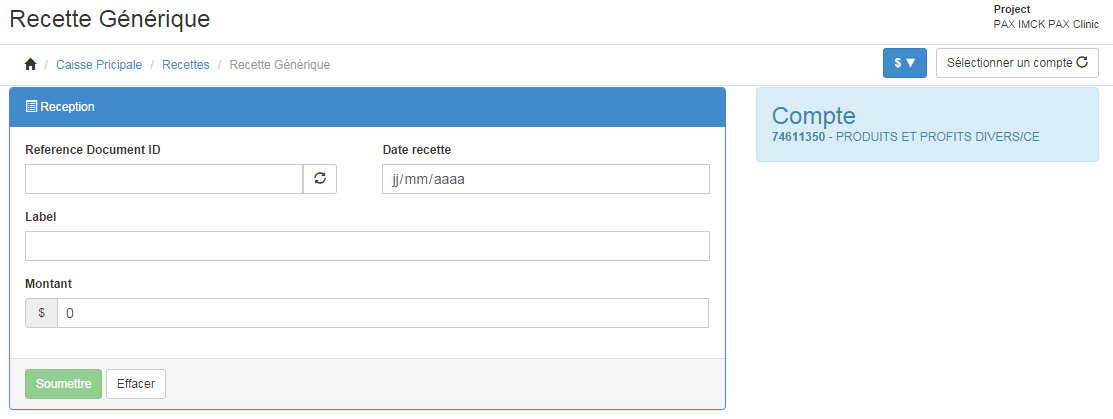
\includegraphics[width=14cm]{pic/recetteGen2.png}
\end{center}
\caption{Interface principale permettant d'enregistrer une recette générique}
\label{Interface principale permettant d'enregistrer une recette générique}
\end{figure}

Dans la zone qui retrouve à droite renseigne sur le compte qui est utilé pour l'opération. Il suffit de cliquer sur le bouton soumettre pour confirmer l'enregistrement de la dépense.

\begin{figure}[h]
\begin{center}
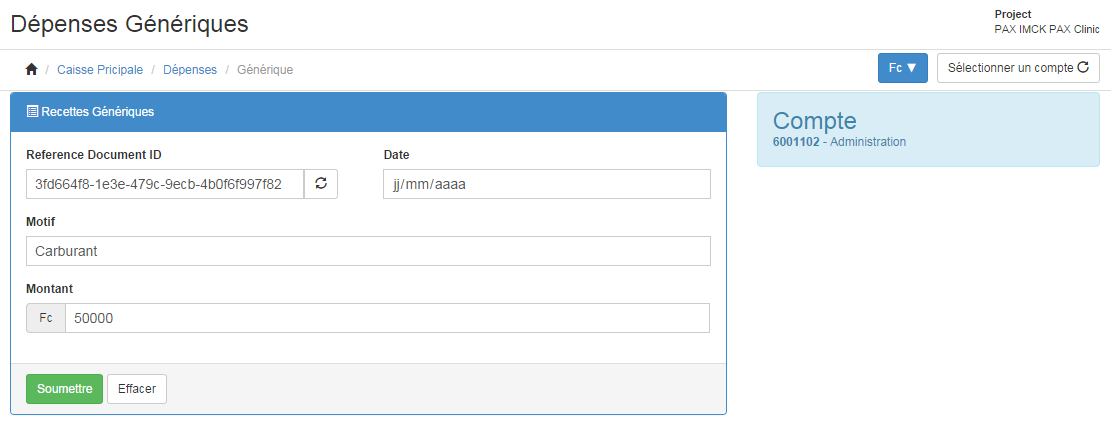
\includegraphics[width=14cm]{pic/FormDepGen.png}
\end{center}
\caption{Apperçue de l'utilisisation du dépense générique}
\label{Apperçue de l'utilisisation du dépense générique}
\end{figure}


\newpage
\chapter{Le module Rapports}        
%////////////////////////////////////////////////%
Le module rapports permet de pouvoir visualiser plusieurs types des rapports résultants du fonctionnements du système, La figure ci-dessous représente avec exactitude ce module avec les différents sous éléments.

\begin{figure}[h]
\begin{center}
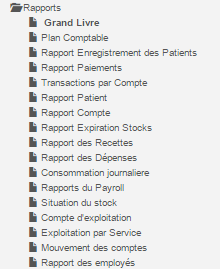
\includegraphics[width=4cm]{pic/ArboReport.png}
\end{center}
\caption{Arborescence du module Rapports}
\label{Arborescence du module Rapports}
\end{figure}
\newpage
\section{Plan Comptable}
Le plan comptable permet la visualisation du plan comptable et donne la possibilité de pouvoit imprimer le plan comptable. L'interface principale de ce module se présente de la manière suivante. 

\begin{figure}[h]
\begin{center}
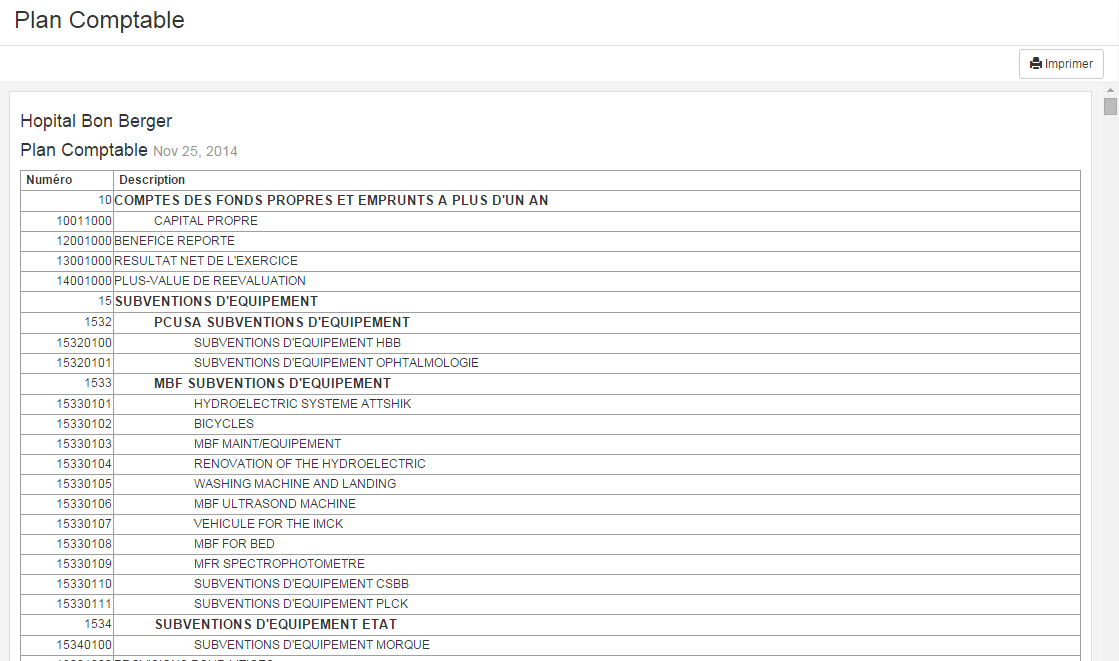
\includegraphics[width=14cm]{pic/PlanComptableAf.png}
\end{center}
\caption{Aperçue du Plan Comptable}
\label{Aperçue du Plan Comptable}
\end{figure}

\newpage

\newpage
\section{Rapport Paiements}
Le rapport de paiement permet de visualiser l'historique de paiement s'éffectuant aux niveaux des caisses auxilliaires dans le système. L'interface principale permettant de voire le rapport de paiements se présente de la manière suivante. 

\begin{figure}[h]
\begin{center}
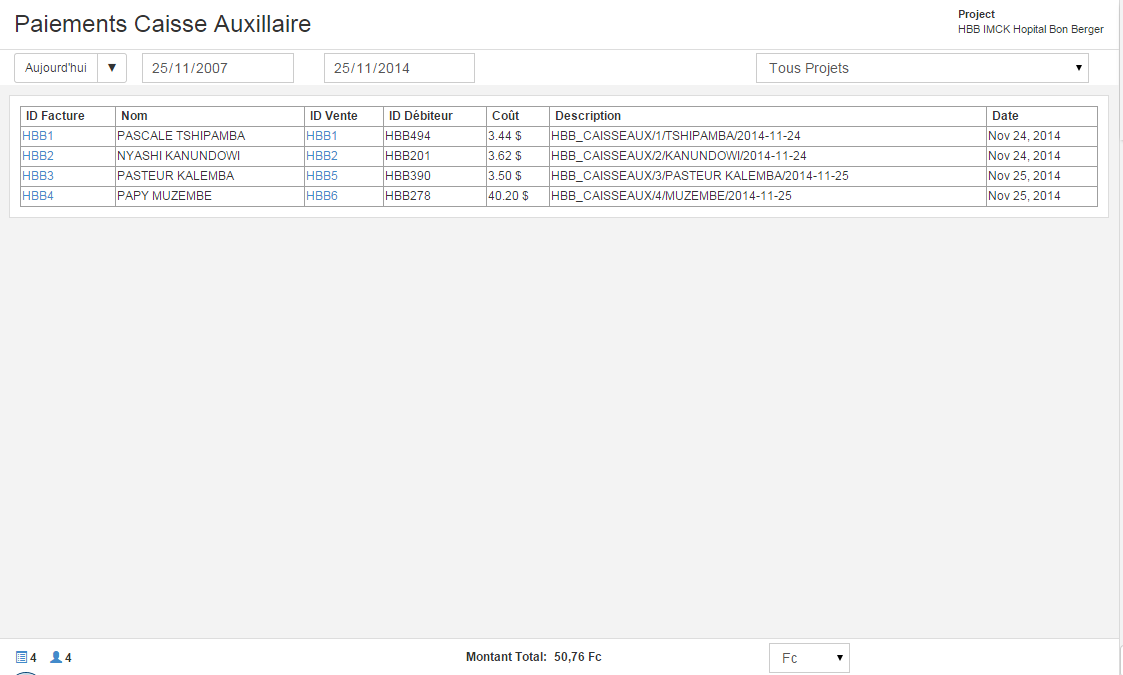
\includegraphics[width=10cm]{pic/rapportCaisseAux.png}
\end{center}
\caption{Aperçue de l'interface principale du rapport de paiements}
\label{Aperçue de l'interface principale du rapport de paiements}
\end{figure}

Par défaut le rapport de paiement affiche la liste des paiements effectués le jour courant, l'interface du rapport d'enregistrement dispose de plusieurs outils permettant de visualiser les anciens paiements répertories.

Le bouton 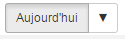
\includegraphics[scale=0.7]{pic/Todays.png} donne la possibilité de visualiser les paiements du jour courant, de la semaine courante mais aussi ceux du mois courant. 

Il existe aussi  
\includegraphics[scale=0.7]{pic/PlageTimes.png} qui permet visualiser le rapport de paiement en precisant une plage de valeur entre deux dates.

Il existe aussi une liste de choix qui donne la possibilité de visualiser le rapport d'enregistrement par projets ou bien de tous le projet à la fois.

En bas de page on retrouve les indicateurs sur le rapport de paiements, on retrouve le nombre des paiements qu'il y'a eu ainsi que le montant total des paiements ainsi que la possibilité de visualier le total avec différentes monnaies. 

\begin{figure}[h]
\begin{center}

\includegraphics[width=9cm]{pic/IndRapPaiement.png}
\end{center}
\caption{Aperçue des indicateurs du rapport de paiements}
\label{Aperçue des indicateurs du rapport de paiements}
\end{figure}


\newpage
\section{Rapport des Recettes}
Le rapport des recettes permet de visualiser toutes les entrés en caisse qui s'éffectue aux niveaux de la caisse principale, l'interface principale de ce module se présente de la manière suivante.

\begin{figure}[h]
\begin{center}
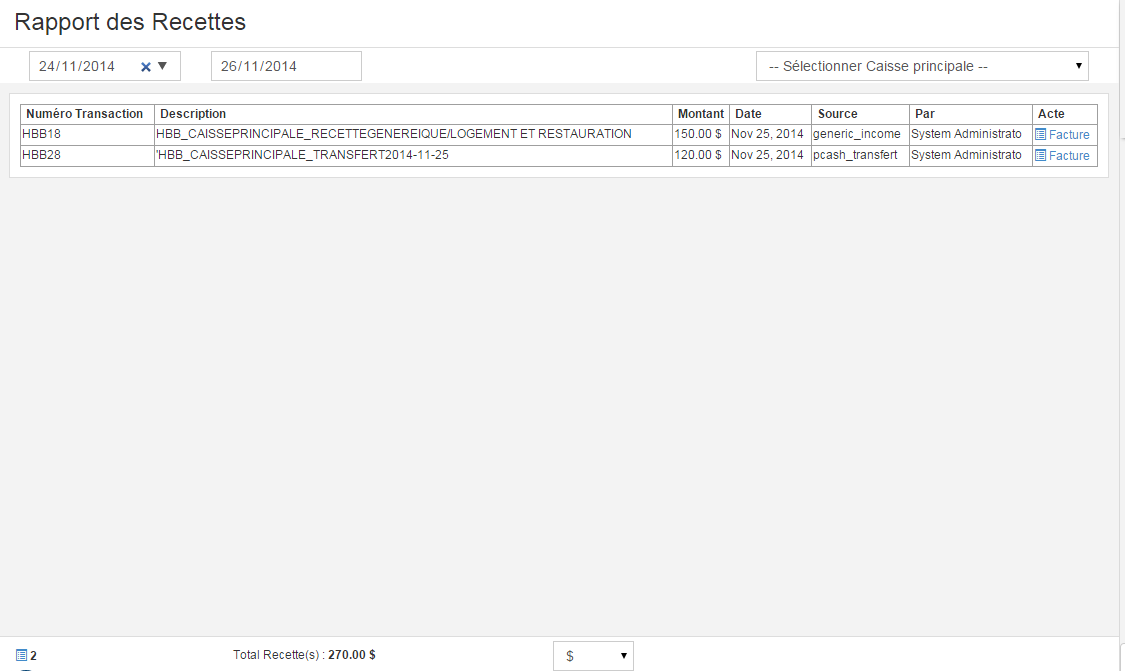
\includegraphics[width=14cm]{pic/RapportRecette.png}
\end{center}
\caption{Interface principale du module Rapport des recettes}
\label{Interface principale du module Rapport des recettes}
\end{figure}

La zone  
\includegraphics[scale=0.7]{pic/PlageTimes.png} qui permet visualiser le rapport des recettes en précisant une plage de temps par rapport aux dates.

Dans le tableau des recettes il existe le lien 
\includegraphics[scale=0.7]{pic/FactureRePrint.png} qui permet de réafficher les détailles d'une recette.

Il est aussi possible de pouvoir choisir les recettes respectivement par rapport à la monnaie qui a été utilisé au moment de la transaction grace à la liste de choix 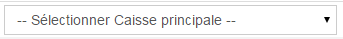
\includegraphics[scale=0.7]{pic/SelecPriCash.png}.

En bas de page on retrouve les indicateurs permettant de connaitre le nombre des recettes qui ont été réaliser ainsi que le montant total des recettes ainsi que la possibilité de le visualiser avec différentes monnaies. 

\newpage
\section{Rapport des Dépenses}
Le rapport des dépenses permet de visualiser toutes les sorties en caisse qui s'éffectue aux niveaux de la caisse principale, l'interface principale de ce module se présente de la manière suivante.

\begin{figure}[h]
\begin{center}
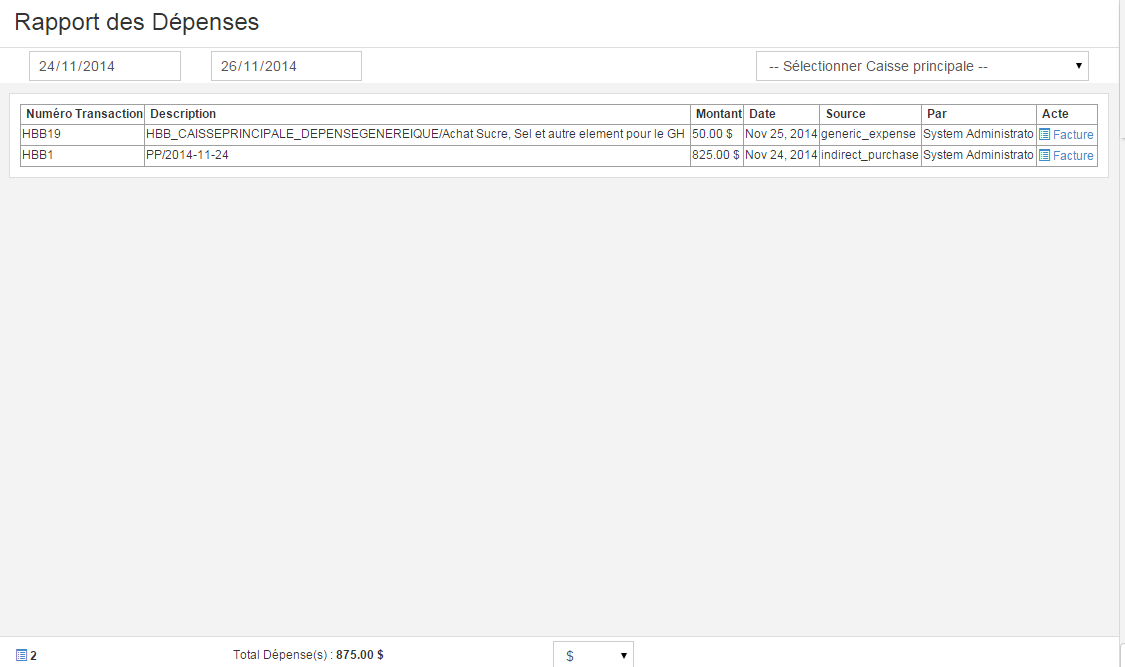
\includegraphics[width=14cm]{pic/RapDepenses.png}
\end{center}
\caption{Interface principale du module Rapport des dépenses}
\label{Interface principale du module Rapport des dépenses}
\end{figure}

La zone  \includegraphics[scale=0.7]{pic/PlageTimes.png} qui permet visualiser le rapport des dépenses en précisant une plage de temps par rapport aux dates.

Dans le tableau des dépenses il existe le lien \includegraphics[scale=0.7]{pic/FactureRePrint.png} qui permet de réafficher les détailles d'une dépense.

Il est aussi possible de pouvoir choisir les depenses respectivement par rapport à la monnaie qui a été utilisé au moment de la transaction grace à la liste de choix \includegraphics[scale=0.7]{pic/SelecPriCash.png}.

En bas de page on retrouve les indicateurs permettant de connaitre le nombre des recettes qui ont été réaliser ainsi que le montant total des recettes ainsi que la possibilité de le visualiser avec différentes monnaies. 


%%%%%%%%%%%%%%%%%%%%%%%%%%%%%%%%%%%%%%%%%%%%%%%%%
% Table des matieres
\tableofcontents
\end{document}